% GENERATED FROM typst/manual/sections/00_scope.typ BY scripts/typ2tex.py (v1.0.0) — DO NOT EDIT.
% Edit canonical Typst under typst/ and regenerate with: python3 scripts/typ2tex.py --root . --outdir latex

\section{Scope}\label{manual:scope}

This manual carries application and prediction-test material downstream from the main A$\Omega$D note. The main note carries the AF/AFC/A$\Omega$D calculus. This manual carries calculation records, setup diagrams, comparison targets, external-comparison records, error audits, and audit tables.

\subsection{Use of this manual}\label{manual:scope:use}

The manual uses the same section / subsection / subsubsection structure as the main note. Rest-energy calculation records are organized under \secref{manual:rest-energy-prediction}. External comparison material remains downstream and quarantined from the A$\Omega$-internal scoped-flux calculation.

\subsection{Simulation reading route}\label{manual:simulation-reading-route}

Follow Main in its dependency order: specific distinction, closure and recurring wave, motif/field folding, complete wave state and relational time, then Stokes/SADAR/harmonic values. Manual Scope is followed by the consolidated native fixtures, the D.E.C. ledger and the retained applications.

\subsection{Calculation spine}\label{manual:calculation-spine}

The common method has five operations. Declare the setup: retained fields,
ancestry, window, boundary, coupled and shed currents, and update law. Admit
source-bound inputs with their roles, acquisition maps and uncertainty.
Compute on that setup, retaining the state needed by its dynamics. Map the
outputs with the declared observation, clock and calibration. Finally join
the frozen comparison evidence, propagate shared dependencies and challenge
the stated claim. Applications below supply their choices and exact values;
the measures and mappings chapters own the map and uncertainty calculations.

The manual uses one active calculation language. A calculation declares

\[
B=(\partial_TF,\omega).
\]

It forms retained cycle provenance, evaluates branch/hinge/branch, and computes a SADAR value:

\[
C_f[\Sigma]_{\AO},\qquad\mathsf{AO}_{\mu}(C)=\langle\Pi_{\alpha},H_{\mu},\Pi_{\Omega}\rangle,\qquad\SADARop_B(C)=p^D_{C,\AO}A_{C,\AO}.
\]

The boundary value is stored by

\[
\Phi^D_{\partial_TR}=\sum_{e\in\partial_TR}\SADARop_B(C_e).
\]

Tables store evaluated values. Tables are not the calculus.

\subsection{Worked-calculation release}\label{manual:worked-calculation-release}

A worked record follows one sequence: question, dependencies, cited input,
declared reduction, local choices, operator chain, exact block, intermediate
table, exact output row, exact-to-report map, comparison, figure,
reproducibility, and falsification hook. Its opening calculation card names
the supplied stages and the unresolved obligations; the detailed calculation
and authoritative tables remain with the application.

For an exact A$\Omega$-internal fixture, form

\[
\text{setup}\to A{\leftrightarrow}_{\mu}\Omega\text{ calculation}\to\text{fixture comparator}\to\Delta^{\mathbb{Z}},\delta_3\to\text{audit}.
\]

For an external comparison calculation, form

\[
\text{setup}\to A{\leftrightarrow}_{\mu}\Omega\text{ calculation}\to\text{observable / target record}\to\Delta,\epsilon,z,\sigma\to\text{error audit}.
\]

The symbols $\Delta$, $\epsilon$, $z$, and $\sigma$ belong to the external comparison layer. A target-only pull uses the declared target standard uncertainty and is
labelled $z_{\mathrm{target}}$. A standardized joint residual additionally
requires the uncertainty of both sides and their dependence.

For a benchmark-dataset calculation, record

\[
\mathbf{a}\vdash(F,R,\partial_TR,\omega),\quad\mathcal{D}_{\mathrm{bench}},\quad\mathcal{Q}_{\mathrm{required}},\quad\mathcal{S}=\text{benchmark manifest}.
\]

Registry rows carry benchmark calculations until the declared dataset, required coordinate, report map, and audit fields are supplied.

\aodnoteblock{Placement rule}{A worked record carries a complete simulation or comparison row. Registry rows carry declared setup, target, comparator, residual, uncertainty, and audit fields as they are supplied.}

\aodnoteblock{Specification discipline}{A rest or prediction record may use a compact curling-curl specification only after $HT(K;B)$ is declared or inherited.}

\subsection{Table discipline}\label{manual:table-discipline}

Tables retain evaluated values, targets, residuals and their provenance. The calculation is the declared boundary computation

\[
\mathbf{a}\vdash(F,R,\partial_TR,\omega),\qquad B=(\partial_TF,\omega),
\]

followed by the A$\Omega$ and SADAR calculation on that boundary.

\subsection{Provenance-label policy}\label{manual:provenance-label-policy}

Tokens of the form \texttt{main:<anchor>} and \texttt{manual:<anchor>} are cross-document provenance anchors. They refer to the corresponding source label \texttt{<anchor>} in the named document. Reader pointers render the published equation, section, appendix or table number from that label; the full source keys remain in macro arguments or source metadata. Explicit alias labels declare alternate anchors. Provenance records remain internal-reference lists; external sources belong in Literature note records.

\subsection{Exact arithmetic and presentation decimals}\label{manual:exact-arithmetic-presentation}

A$\Omega$-internal calculations use integer counts and exact rational ratios. Decimal values appear only as external comparison coordinates, presentation values, or plot labels.

\[
\text{A}\Omega\text{ side: integers / fractions},\qquad\text{external side: value }\pm\text{ declared uncertainty}.
\]

If an external measured decimal is used as a comparison target, the comparison record declares its uncertainty $\sigma$ when a $z$-score is formed. Percent errors may be shown as presentation comparisons when the target value is declared.

\subsubsection{Exact-fixture corollary}\label{subsec:frg-delta-three-corollary}

If an exact fixture declares

\[
T_k^{\times},O_k\in\mathbb{Z},
\]

then record the exact ternary signed residual

\begin{equation}\label{eq:frg-delta-three-components}
\Delta_k^{\mathbb{Z}}=T_k^{\times}-O_k,\qquad s_k^{(3)}=\operatorname{sgn}(\Delta_k^{\mathbb{Z}})\in\{-1,0,+1\},\qquad m_k=|\Delta_k^{\mathbb{Z}}|\in\mathbb{Z}_{\ge0}.
\end{equation}

Thus

\begin{equation}\label{eq:frg-delta-three-signed-product}
\Delta_k^{\mathbb{Z}}=s_k^{(3)}m_k.
\end{equation}

The compact residual package is

\begin{equation}\tag{RG10}\label{eq:frg-delta-three}
\delta_{3,k}(T^{\times},O)=(s_k^{(3)},m_k),\qquad\delta_3(T^{\times},O)=(\delta_{3,k}(T^{\times},O))_{k\in K_{\mathrm{bin}}}.
\end{equation}

Normalized decimal summaries belong to declared value maps or external comparison entries.

SYM-A5 checks integer-fixture residuals \eqref{eq:frg-delta-three}.
RG-A10 forms $T_k^{\times}-T_k^0=\sum C_{ij,k}^{\times}(B)$ for
declared exact integer fixtures. RG-A11 records $\Delta^{\mathbb{Z}}$ and
$\delta_3$ using \eqref{eq:frg-delta-three-components}--\eqref{eq:frg-delta-three}.

\aodnoteblock{Decimal precision record}{A released decimal presentation value carries

\[
(x_{\mathrm{disp}},u_x,\mathrm{unit}(x),\mathrm{src}(x),\mathrm{round}(x),\mathrm{scope}(x)).
\]

Here $\mathrm{scope}(x)\in\{\text{internal},\text{external},\text{measured},\text{derived external},\text{value map},\text{demonstration}\}$. The precision field $u_x$ records declared display uncertainty.}

\subsection{External-comparison quarantine}\label{manual:external-comparison-quarantine}

Measured preparation or boundary inputs may enter through declared acquisition
or reduction maps, with their source assumptions and uncertainty retained.
External laws and constants do not thereby become calculus premises or set
native notation. Calibration inputs and evaluation targets have separate
roles; target exposure during selection remains part of the record. In this manual, an external comparison is written

\[
\Qext(\nu_{x,\AO};\mathcal{T}_x),
\]

where $\mathcal{T}_x$ is a declared measured-sector target record.

\subsection{Scoped errors by data-support class}\label{manual:scoped-errors-data-support}

For $r=y_{\mathrm{model}}-y_{\mathrm{observed}}$, the joint variance in
\eqref{eq:manual-m3-residual-dependence} retains shared sources across both sides. Exact
finite laws permit evaluation at every input case; affine maps permit exact
propagation of complete moments; justified intervals give bounds. A nonlinear
moment-only calculation is a linearized diagnostic unless its remainder is
bounded. A source-reported uncertainty alone supplies no probability law.
Unknown components remain unknown; display rounding and exact conditional
arithmetic do not establish physical certainty.

A simulation or comparison is classified by the declared data support it instantiates. Dataset resolution selects the data-support class: radial rows instantiate G0; radial rows plus proxy density/current fields instantiate G1; three-dimensional density/velocity/current fields instantiate G2; time-ordered tracer positions/velocities instantiate G3. Each class reports residuals in its declared coordinate. Projection and marginalization maps carry their own comparison coordinates and uncertainty records.

The scoped-error chain is

\[
D\to R(D)\to\mathcal{M}(D,R)\to\Pi_{\mathrm{report}}\to\epsilon_{\mathrm{report}}.
\]

Here $D$ is the declared data-support distinction layer, $R(D)$ is the induced relation family, $\mathcal{M}(D,R)$ is the AFC/A$\Omega$D model evaluated on that cut, $\Pi_{\mathrm{report}}$ is the report or projection map, and $\epsilon_{\mathrm{report}}$ is the residual relative to the declared output target. Every manual comparison declares its data-support class before residuals are interpreted.

\paragraph{Simulation data card.}
Each simulation or comparison row records

\[
(D,C_{\mathrm{support}},M_{\AO},\Pi_{\mathrm{report}},\sigma_{\mathrm{input}},\epsilon_{\mathrm{report}},\mathrm{src}).
\]

Here $D$ is the declared input data, $C_{\mathrm{support}}$ is the data-support class, $M_{\AO}$ is the AFC/A$\Omega$D calculation or map, $\Pi_{\mathrm{report}}$ is the reported coordinate, $\sigma_{\mathrm{input}}$ is the declared input uncertainty when present, $\epsilon_{\mathrm{report}}$ is the residual/error coordinate, and $\mathrm{src}$ records the data source or source artifact.

\subsection{Manual record forms}\label{manual:record-forms}

Each application card binds its question, fields/window/boundary, inherited
construction and local choices, input roles, exact calculation, observation
and clock, comparison, and falsifier. The associated quantity rows use this
compact form; detailed source identities and covariance remain in the bound
comparison record.

\begin{center}
{\footnotesize
\begin{tabularx}{\linewidth}{l>{\raggedright\arraybackslash}X>{\raggedright\arraybackslash}X>{\raggedright\arraybackslash}X>{\raggedright\arraybackslash}X}
\toprule
Quantity/role & Source and unit/domain & Value/state & Uncertainty and shared sources & Map and unresolved input \\
\midrule
Preparation & Exact, measured or derived & Admitted input & Law, moments, bound or unknown & Acquisition/reduction \\
Output & Named conditional law & Computed value & Propagated inputs and map & Model/reduction remainder \\
Target & Evaluation or development & Source value & Measurement and shared calibration & Observation reduction \\
Residual & Named comparison & Difference/statistic & Joint result or partial diagnostic & Missing dependence \\
\bottomrule
\end{tabularx}
}
\end{center}

An exact fixture specifies exact operands; physical preparation and
observation uncertainties are uninstantiated until a physical application
supplies them. Data support, supplied stages, replay and empirical evidence
are recorded separately in \secref{manual:prediction-test-registry}.

\begin{table}[H]
\centering
\caption{Manual record forms.}
\label{tab:manual-record-forms}
{\footnotesize
\begin{tabularx}{\linewidth}{l>{\raggedright\arraybackslash}X}
\toprule
Record form & Active fields \\
\midrule
A$\Omega$ field record & support, carried cycle, pressure/accessor values, and retained A$\Omega$ value \\
Measured target record & target value, declared uncertainty, measured-sector coordinate, and citation \\
External comparison record & map value, target, residual/error coordinate, uncertainty source, and audit hook \\
Observable-map record & observable-map value, target, residual, percent error, citation, and audit hook \\
Exact fixture & comparator bins, $\Delta^{\mathbb{Z}}$, $\delta_3$, closure residual, and sheddic-route audit \\
Benchmark manifest & dataset table, required report coordinate, input data sources, and audit hook \\
Calibration anchor & convention value and convention-audit residual \\
\bottomrule
\end{tabularx}
}
\end{table}

\paragraph{Construction and record classes.}
Native fixtures establish exact typed relations; declared models specify their
chosen update/coupling law; metrology records add calibration and units;
empirical comparisons additionally bind external data and residuals. Admission
precedes all four projections. The common construction is distinction,
retained relation, admitted motif/closure, recurring wave, scoped field
organization, complete state/trace and native comparison. A field resolves
wave identities and is not retained closure lineage itself. Motion is the
later realized pressure-bearing transition. Modular coordinate phase in the
3D applications is a downstream statistic; sampling interval is an acquisition
coordinate. Native closure counts and RCD are not measured time.

\subsection{Five-boundary D.E.C. execution spine and chapter index}\label{manual:scope:five-boundary-spine}

Every worked example across this manual instantiates one uniform five-boundary execution spine on an explicit finite support $R$, its typed boundary $\partial_TR$, and an integer window $\omega$:

\[
B_{\mathrm{in}}\to B_{\mathrm{core}}\to B_{\mathrm{shed}/\mathrm{slide}}\to B_{\mathrm{sensor}}\to B_{\mathrm{ext}}=\mathsf{Q}_{\mathrm{ext}}.
\]

Zero-float evaluations execute in both the Python reference engine (\texttt{python3 -B -m manual.engine --sector boundary\_sadar}) and the Rust exact core (\texttt{aod-core --verify-vectors --check-zero-float}) across all fifty-three locked golden vectors---\texttt{RC-001} through \texttt{RC-045} ($45$ \texttt{rational\_core}) and \texttt{SD-001} through \texttt{SD-008} ($8$ \texttt{symbolic\_and\_display}). No floating-point value, background continuum clock, or external SI constant enters $B_{\mathrm{in}}\to B_{\mathrm{sensor}}$.

\begin{figure}[H]
\centering
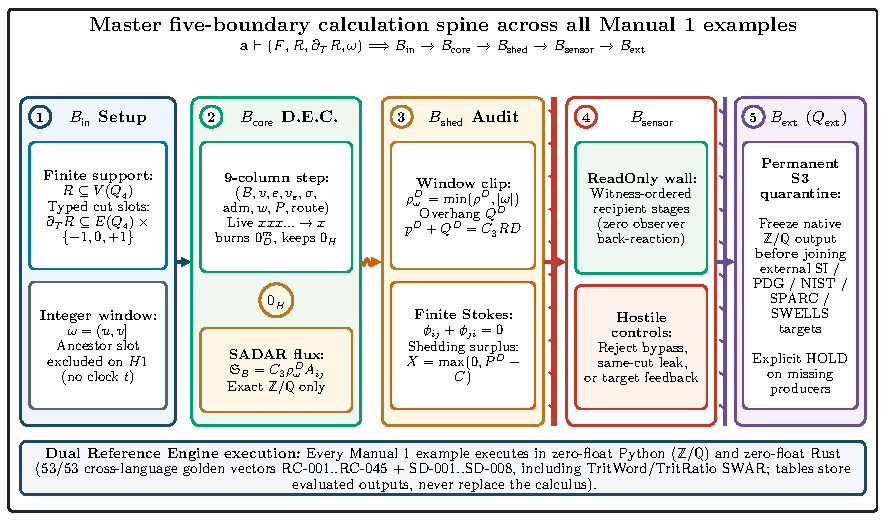
\includegraphics[width=0.92\linewidth,height=0.78\textheight,keepaspectratio]{figures/generated/five-boundary-calculation-spine.pdf}
\caption{Five-boundary D.E.C. calculation spine $B_{\mathrm{in}}\to B_{\mathrm{core}}\to B_{\mathrm{shed}/\mathrm{slide}}\to B_{\mathrm{sensor}}\to B_{\mathrm{ext}}=\mathsf{Q}_{\mathrm{ext}}$ binding all Manual sections and appendices to the zero-float reference engines.}
\label{fig:manual-five-boundary-calculation-spine}
\end{figure}

\begin{table}[H]
\centering
\caption{Uniform five-boundary D.E.C. calculation index across Manual sections and appendices.}
\label{tab:manual-chapter-dec-boundary-index}
{\scriptsize
\begin{tabular}{>{\raggedright\arraybackslash}p{0.138\linewidth}>{\raggedright\arraybackslash}p{0.294\linewidth}>{\raggedright\arraybackslash}p{0.184\linewidth}>{\raggedright\arraybackslash}p{0.304\linewidth}}
\toprule
Unit & Declared 5-boundary stack & Engine vectors & Frozen D.E.C. / SADAR artifact \\
\midrule
\S2 Closure \& wave & $B_{\mathrm{monon}}\to B_{\mathrm{asym}}\to B_{\mathrm{wave}}\to B_{\mathrm{fold}}\to B_{\mathrm{harm}}$ & \texttt{RC-033} & \texttt{native\_\allowbreak{}closure\_\allowbreak{}wave\_\allowbreak{}dec\_\allowbreak{}walk.csv} \\
\S3 Operativity & $B_{\mathrm{shared}}\to B_{S^+}\to B_{S^{-e}}\to B_{\mathrm{sensor}}\to B_{\mathrm{hold}}$ & \texttt{RC-034} & \texttt{awareness\_\allowbreak{}operativity\_\allowbreak{}dec\_\allowbreak{}walk.csv} \\
\S4 D.E.C. ledger & $B_{\mathrm{in}}\to B_{\mathrm{flip}}\to B_{\mathrm{slide}}\to B_{\mathrm{disoma}}\to B_{\mathrm{ext}}$ & \texttt{RC-025}, \texttt{RC-026}, \texttt{RC-045} & \texttt{dec\_\allowbreak{}chiral\_\allowbreak{}flip\_\allowbreak{}continuous\_\allowbreak{}walk.csv}, \texttt{ternary\_\allowbreak{}swar\_\allowbreak{}and\_\allowbreak{}trit\_\allowbreak{}ratio} \\
\S5 Cell measures & $B_{\mathrm{cell}}\to B_{\mathrm{stair}}\to B_{\mathrm{fold}}\to B_{\mathrm{audit}}\to B_{\mathrm{ext}}$ & \texttt{RC-035} & \texttt{cell\_\allowbreak{}measures\_\allowbreak{}staircase\_\allowbreak{}fold\_\allowbreak{}dec.csv} \\
\S6 Typed maps & $B_{\mathrm{src}}\to B_{\mathrm{map}}\to B_{\mathrm{joint}}\to B_{\mathrm{role}}\to B_{\mathrm{ext}}$ & \texttt{RC-036} & \texttt{typed\_\allowbreak{}map\_\allowbreak{}joint\_\allowbreak{}law\_\allowbreak{}ledger.csv} \\
\S7 Temporal \& SI & $B_{\mathrm{pair}}\to B_{\mathrm{lag}}\to B_{\mathrm{bridge}}\to B_{\mathrm{val}}\to B_{\mathrm{ext}}$ & \texttt{RC-037} & \texttt{temporal\_\allowbreak{}si\_\allowbreak{}bridge\_\allowbreak{}dec\_\allowbreak{}ledger.csv} \\
\S8 Short-window & $B_{\mathrm{core}}\to B_{\omega}\to B_{\mathrm{close}}\to B_{\mathrm{shed}}\to B_{\mathrm{ext}}$ & \texttt{RC-030}, \texttt{RC-038} & \texttt{dimonhexon\_\allowbreak{}double\_\allowbreak{}slit\_\allowbreak{}ring\_\allowbreak{}paths.csv}, \texttt{short\_\allowbreak{}window\_\allowbreak{}rcd\_\allowbreak{}dec\_\allowbreak{}ledger.csv} \\
\S9 Rest energy & $B_{\mathrm{hard}}\to B_{\tau}\to B_{\mathrm{shed}}\to B_{\mathrm{sensor}}\to B_{\mathrm{ext}}$ & \texttt{RC-027}--\texttt{RC-029}, \texttt{SD-007} & \texttt{tau\_\allowbreak{}five\_\allowbreak{}boundary\_\allowbreak{}sadar\_\allowbreak{}trace.csv}, \texttt{higgs\_\allowbreak{}baryon\_\allowbreak{}overlap\_\allowbreak{}saddle\_\allowbreak{}scan.csv}, \texttt{rest\_\allowbreak{}energy\_\allowbreak{}sadar\_\allowbreak{}debris\_\allowbreak{}atlas.csv} \\
\S10 Hydrogen & $B_{\mathrm{core}}\to B_{S_n}\to B_{S_m}\to B_{\mathrm{sensor}}\to B_{\mathrm{ext}}$ & \texttt{RC-031}, \texttt{RC-039} & \texttt{hydrogen\_\allowbreak{}shell\_\allowbreak{}exact\_\allowbreak{}series.csv}, \texttt{hydrogen\_\allowbreak{}shell\_\allowbreak{}dec\_\allowbreak{}transitions.csv} \\
\S11 Wire \& Stokes & $B_{\mathrm{wire}}\to B_e\to B_{\mathrm{int}}\to B_{R_1\cup R_2}\to B_{\mathrm{ext}}$ & \texttt{RC-032} & \texttt{scoped\_\allowbreak{}wire\_\allowbreak{}and\_\allowbreak{}moving\_\allowbreak{}boundary\_\allowbreak{}walk.csv} \\
\S12 Solar O0 & $B_{\mathrm{Sun}}\to B_{\mathrm{Hg/bend/red}}\to B_{\mathrm{gate}}\to B_{\mathrm{O0}}\to B_{\mathrm{ext}}$ & \texttt{RC-040} & \texttt{solar\_\allowbreak{}o0\_\allowbreak{}boundary\_\allowbreak{}dec\_\allowbreak{}audit.csv} \\
\S13 Field dynamics & $B_{Q_4}\to B_{\mathrm{hinge}}\to B_{\mathrm{ring}}\to B_{\mathrm{pool}}\to B_{\mathrm{ext}}$ & \texttt{RC-041}, \texttt{SD-008} & \texttt{run\_\allowbreak{}tumble\_\allowbreak{}q4\_\allowbreak{}dec\_\allowbreak{}walk.csv}, \texttt{sparc\_\allowbreak{}pooled\_\allowbreak{}primary\_\allowbreak{}exact.csv} \\
\S14 Lensing plan & $B_{\mathrm{src}}\to B_{\mathrm{shell},k}\to B_{\mathrm{FRG}}\to B_{\delta_3}\to B_{\mathrm{SWELLS}}$ & \texttt{RC-020}, \texttt{RC-042} & \texttt{lensing\_\allowbreak{}ray\_\allowbreak{}chiral\_\allowbreak{}dec\_\allowbreak{}walk.csv} \\
App. A Shedding & $B_{\mathrm{span}}\to B_{\mathrm{clip}}\to B_{\mathrm{shed}}\to B_{\mathrm{reclose}}\to B_{\mathrm{ext}}$ & \texttt{RC-014}, \texttt{RC-043} & \texttt{cycle\_\allowbreak{}shedding\_\allowbreak{}exact\_\allowbreak{}rational\_\allowbreak{}summary.csv} \\
App. B Quarantine & $B_{\mathrm{core}}\to B_{\mathrm{sensor}}\to B_{\mathrm{map}}\to B_{\mathrm{tar}}\to\mathsf{Q}_{\mathrm{ext}}$ & \texttt{SD-007} & \texttt{rest\_\allowbreak{}energy\_\allowbreak{}sadar\_\allowbreak{}debris\_\allowbreak{}atlas.csv} \\
App. C 3D phase & $B_{\mathbb{Z}^3}\to B_{\mathrm{lag}}\to B_{\mathrm{phase}}\to B_{\mathrm{oct}}\to B_{\delta_3}$ & \texttt{RC-044} & \texttt{coordinate\_\allowbreak{}phase\_\allowbreak{}3d\_\allowbreak{}dec\_\allowbreak{}walk.csv} \\
\bottomrule
\end{tabular}
}
\end{table}
